\chapter{Landmark Graph Construction}
\begin{defn}[\emph{Landmark}]\label{Def:ldmk}
A landmark is a road segment that is frequently traversed by taxi drivers according to the taxi GPS trajectory database. \cite{TDR10}
\end{defn}

The concept of a landmark is proposed primarily for two reasons. First, as mentioned in Section~\ref{Sec:limitation}, the taxi GPS trajectories do not necessarily cover every road segment in a city's road network and the low-sampling-rate problem makes determining the exact route on which a taxi traversed difficult. Therefore, it is not possible to estimate the time cost for each road segment. However, ignoring the length of a road segment and considering it as an abstract ``landmark'' make estimating the travel time between two \emph{landmarks} viable. 

Moreover, the notion of landmarks closely follows the way how drivers remember the driving routes in daily life\cite{TDR10}. For instance, a driving route could be described as ``go straight on the 4th Avenue, turn right at the 7th Street and exit at the Smith Road''. Drivers tend to use familiar road segments as landmarks to guide their directions.

This chapter describes the procedures for constructing a landmark graph in order to estimate the time cost between two landmarks. But before that, the taxi GPS trajectories must be separated into a set of \emph{trips}.

\section{Trip Identification}
\begin{defn}[\emph{Trip}]\label{Def:trip}
A trip is a set of chronologically ordered GPS records belonging to one taxi that satisfies either condition:
\begin{enumerate}
\item A passenger is on the taxi, namely, all records in the set have an OCCUPIED field of value 1 or, 
\item No passenger is on the taxi, but the time difference between \emph{any} two consecutive records is no larger than 3 minutes.
\end{enumerate}
\end{defn}

Table~\ref{Ta:trip_identification} gives a tiny example of trip identification.

\begin{table}[h]
\centering
\resizebox{\columnwidth}{!}{
\begin{tabular}{ | l | l | l | l | l | l | l | l | l | l | l | l | l | }
\hline
\textbf{CUID} & \textbf{UTC} & \textbf{GPS\_LONG} & \textbf{GPS\_LAT} & \textbf{OCCUPIED} & \textbf{TRIP\_ID} \\\hline
1	&	1/5/2009 0:02:00	&	116.39616	&	39.81294	&	0	&	4552265\\ \hline
1	&	1/5/2009 0:04:00	&	116.39575	&	39.82296	&	0	&	4552265\\ \hline
1	&	1/5/2009 0:07:00	&	116.39567	&	39.82774	&	0	&	4552265\\ \hline
1	&	1/5/2009 17:08:00	&	116.30142	&	39.98105	&	1	&	1\\ \hline
1	&	1/5/2009 17:10:00	&	116.29514	&	39.98419	&	1	&	1\\ \hline
1	&	1/5/2009 17:11:00	&	116.28959	&	39.98289	&	1	&	1\\ \hline
1	&	1/5/2009 17:12:00	&	116.28087	&	39.97552	&	1	&	1\\ \hline
1	&	1/5/2009 17:16:00	&	116.26813	&	39.93537	&	1	&	1\\ \hline
1	&	1/5/2009 18:11:00	&	116.36537	&	39.95019	&	0	&	4552271\\ \hline
1	&	1/5/2009 18:12:00	&	116.36546	&	39.94886	&	0	&	4552271\\ \hline
1	&	1/5/2009 18:13:00	&	116.35927	&	39.94528	&	0	&	4552271\\ \hline
\end{tabular}}
\caption{An example of trip identification}\label{Ta:trip_identification}
\end{table}

Clearly, all records in Table~\ref{Ta:trip_identification} belong to one taxi (taxi with CUID = 1) and are sorted chronologically. The first three records, although no passengers are aboard, are considered to be in the same \emph{trip} because the time difference between any two consecutive records is no larger than 3 minute. The next five records constitute another trip, even though the last two records have a time difference of 4 minutes, since a passenger is on the taxi (OCCIPIED = 1). Following the same reasoning as the first three's, the last three records are treated as one trip. Listing~\ref{List:code_trip} gives the pseudocode for trip identification.

\begin{lstlisting}[language = Python, caption = {Pseudocode for trip identification}, label = {List:code_trip} ,frame=single, numbers=left,stepnumber=1]
curr_tripid = 1
last_occup = curr_occup = records[0].OCCUPIED
last_unixepoch = curr_unixepoch = records[0].UNIX_EPOCH
for recd in records:
	curr_occup = recd.OCCUPIED
	curr_unixepoch = recd.UNIX_EPOCH
	if curr_occup != last_occup:
		++curr_tripid
	elif (curr_occup == 0) && \
		(curr_unixepoch - last_unixepoch > threshold):
			++curr_tripid
	recd.TRIP_ID = curr_tripid
	last_occup = curr_occup
	last_unixepoch = curr_unixepoch
\end{lstlisting}

It is noteworthy that although the middle five records with OCCUPIED = 1 come chronologically after the first three records, they are nevertheless assigned a smaller TRIP\_ID. This is due to an adjustment made to the actual implementation of the algorithm. The \emph{actual} algorithm operates in two stages. It first identifies trips for all records with OCCUPIED = 1; only in the second stage does it identify trips for records with OCCUPIED = 0. The rationale for this arrangement is to give priority to the records with passengers aboard, because \textbf{these records are guaranteed to belong to one trip}. In fact, the second condition for identifying trips in Definition~\ref{Def:trip} is more of a heuristic rather than a theorem. It is meant to provide sufficient data for subsequent machine learning tasks with reasonable accuracy.

\section{Landmark Frequency}
Definition~\ref{Def:trip} states that whether recognising a particular road segment as a landmark or not is based on some notion of frequency. Only if a road segment is visited by drivers frequently enough is it recognised as a landmark. In this project, the notion of frequency is given by Definition~\ref{Def:frequency}.

\begin{defn}[\emph{Frequency of a Road Segment}]\label{Def:frequency}
The frequency of a road segment is the sum of \emph{unique} occurrences of that road segment in each trip. 
\end{defn}



\begin{table}[h]
\centering
\resizebox{\columnwidth}{!}{
\begin{tabular}{ | l | l | l | l | l | l | l | l | l | l | l | l | l | }
\hline
\textbf{CUID} & \textbf{UTC} & \textbf{GPS\_LONG} & \textbf{GPS\_LAT} & \textbf{Street} & \textbf{TRIP\_ID} \\\hline
1	&	1/5/2009 0:02:00	&	116.39616	&	39.81294	&	A	&	4552265\\ \hline
1	&	1/5/2009 0:04:00	&	116.39575	&	39.82296	&	A	&	4552265\\ \hline
1	&	1/5/2009 0:07:00	&	116.39567	&	39.82774	&	B	&	4552265\\ \hline
1	&	1/5/2009 17:08:00	&	116.30142	&	39.98105	&	C	&	1\\ \hline
1	&	1/5/2009 17:10:00	&	116.29514	&	39.98419	&	C	&	1\\ \hline
1	&	1/5/2009 17:11:00	&	116.28959	&	39.98289	&	C	&	1\\ \hline
1	&	1/5/2009 17:12:00	&	116.28087	&	39.97552	&	A	&	1\\ \hline
1	&	1/5/2009 17:16:00	&	116.26813	&	39.93537	&	A	&	1\\ \hline
1	&	1/5/2009 18:11:00	&	116.36537	&	39.95019	&	B	&	4552271\\ \hline
1	&	1/5/2009 18:12:00	&	116.36546	&	39.94886	&	C	&	4552271\\ \hline
1	&	1/5/2009 18:13:00	&	116.35927	&	39.94528	&	C	&	4552271\\ \hline
\end{tabular}}
\caption{An illustration of frequency counting}\label{Ta:frequency_count}
\end{table}

Table~\ref{Ta:frequency_count} illustrates how the frequency of a road segment is calculated. In Trip 4552265, Street A occurs twice but \textbf{its frequency increases only by one}. Similarly, Street C occur three times and Street A occur twice in Trip 1, but \textbf{their occurrences only add one to their frequencies}. Therefore, even though Street B \emph{appears} less times than Street A or Street C, \textbf{all streets have the same frequency of 2}, based on this set of records.  

The algorithm for counting frequency of a road segment is rather straightforward as in Listing~\ref{List:code_frequency}.

\begin{lstlisting}[language = Python, caption = {Pseudocode for counting road frequency}, label = {List:code_frequency} ,frame=single, numbers=left,stepnumber=1]
frequencies = dict{}
for trip in trips:
	streets = unique(trip.streets) // get unique streets
	for street in streets:
		if street in frequencies:
			++frequencies[street]
		else:
			frequencies[street] = 1
\end{lstlisting}

\section{Landmark Graph}\label{outlier_detecting}
\subsection{Motivation for Outlier Detection}
The Baidu Maps Web API for reverse geocoding is stable and fast, but does not produce no errors. Sometimes, a GPS data point may be mapped to a main road but actually it is on the side road, which is one of the limitations mentioned in Section~\ref{Sec:limitation} or it is actually mapped to a street that Baidu Maps does not recognise. In neither case will Baidu Maps produce a correct reverse geocoding. Moreover, the reverse geocoding process is asynchronous, which means that it is being performed in the background in parallel with the main application thread. Therefore, it is inevitable that some street names may get lost when the records are being updated or a record is updated with a wrong street name. Figure~\ref{Fig:exmp_outlier} shows a drastic example.

\begin{figure}[h]
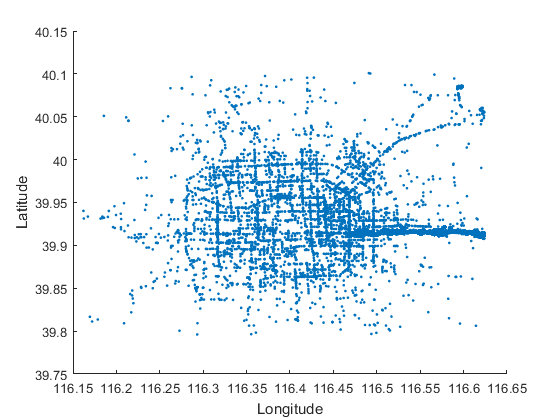
\includegraphics{long_lat_plot}
\centering
\caption{Example of outliers}\label{Fig:exmp_outlier}
\end{figure}

In this example, the Baidu Maps believes that all data points plotted belong to a particular street. But when plotted on a 2-D plane, these data points almost represent the \emph{entire} road network in Beijing. The actual, correct street is represented in the figure as the \emph{thickest} line on the right half of the figure with a longitude ranging from 116.45\textdegree~to 116.65\textdegree.~Erroneous records like those not on the thickest line are known as \emph{outliers} and must be properly identified and removed. This project proposes a novel outlier detection approach based on unsupervised learning whose principle behind is based on Theorem~\ref{Theorem: majority_clustering}.

\begin{defn}[\emph{Reasonable reverse geocoder}]\label{Def:reasonable_geocoder}
A reasonable reverse geocoder always gives its best matching from a GPS data point to a street whenever possible and has an accuracy more than 50\%.
\end{defn}

\begin{theorem}[\emph{Majority Clustering Theorem}]\label{Theorem: majority_clustering}
If a \emph{reasonable reverse geocoder} is used to reverse geocode a set of GPS data points which are mapped to a particular street \emph{in reality}, then, when plotted on a 2-D plane, majority (more than 50\%) of the points must be clustered together to form a rough shape that is similar to the shape of the street that they are supposed to be mapped to. 
\end{theorem}

\begin{proof}
Proof by contradiction. Assume, for the purpose of contradiction, majority (more than 50\%) of the data points that are \emph{indeed} located on the same street are scattered arbitrarily on a 2-D plane after being reverse-geocoded by a reasonable reverse geocoder. In particular, when plotted on a 2-D plane, majority of them do not form a similar shape to that of the street they are supposed to be mapped to. Then, the majority must have been erroneously mapped to some other streets because no single street covers the whole city area. Thus, the reasonable reverse geocoder has only achieved an accuracy less 50\%, which contradicts the Definition~\ref{Def:reasonable_geocoder} of a reasonable reverse geocoder. 
\end{proof}

\subsection{Outlier Identification}
Apparently, Baidu Maps provides a reasonable reverse geocoder because it is of industrial-grade quality and has an accuracy larger than 50\%. Therefore, if a set of points belong to a particular street, after reverse-geocoded by Baidu Maps, majority of them should be clustered to assume a rough shape of that street according to Theorem~\ref{Theorem: majority_clustering}. Based on that, an unsupervised learning technique --- clustering can be used to separate the correctly mapped data points from outliers. 

Many clustering techniques are available\cite{LO05}. Since each record can be represented graphically by a point on a 2-D plane with longitute as the $x$ axis and latitude as the $y$ axis, a \textbf{self-organising feature map}\cite{TK82}(SOFM) seems to be an appropriate technique to use. 

\begin{figure}[h]
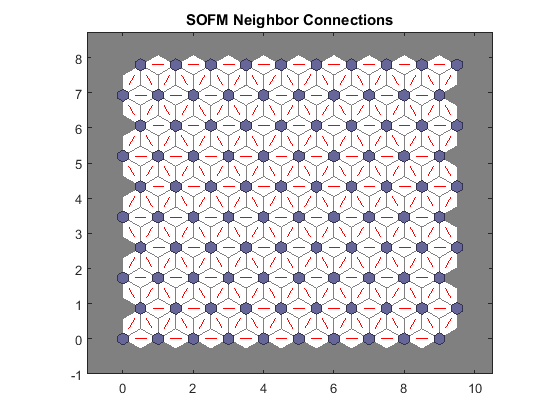
\includegraphics{neighbour_connections}
\centering
\caption{An example of SOFM}\label{Fig:neighbour_connections}
\end{figure}

A self-organising feature map is a form of artificial neural network. It consists of a pre-defined number of interconnected neurons distributed over a 2-D plane as shown in Figure~\ref{Fig:neighbour_connections}. Prior to training, the neurons are randomly scattered among the data points and gradually move to the centroids of the data clusters they represent as they learn the \emph{features} of the training data. Upon termination of the training, all data points near to a particular neuron, in terms of Euclidean distance\footnote{Other distance measures are also possible.}, are assigned to the cluster that neuron represents. Figure~\ref{Fig:sofm_weights} shows the results after the clustering is completed. 

\begin{figure}[h]
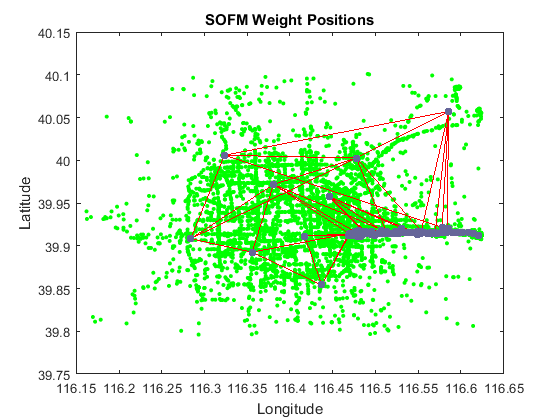
\includegraphics{sofm_weights}
\centering
\caption{Neuron positions after training}\label{Fig:sofm_weights}
\end{figure}

It is clear from the figure that while some neurons represent the clusters of outliers, majority of the neurons are clustered to \emph{cover} the correct street they should represent. A $10\times10$ SOFM was used in this project, so there were at most 100 neurons or equivalently, 100 clusters. Each cluster had a different size. To ensure a thorough removal of the outliers, \textbf{only the top 50\% largest clusters were considered as clusters of correct data points which are called ``legal clusters''. All other clusters were deemed as clusters of outliers}. 

\subsection{Outlier Removal}
Once the legal clusters were identified, a distance threshold was set to remove outliers so that \textbf{whenever the minimum distance between a data point and all centroids of the legal clusters was above the threshold, that data point would be considered as an outlier and removed}. The python-like pseudocode in Listing~\ref{List:code_outlier} describes this idea with more clarity.

%\begin{minipage}{\linewidth}
\begin{lstlisting}[language = Python, caption = {Pseudocode for outlier detection}, label = {List:code_outlier} ,frame=single, numbers=left,stepnumber=1]
for record in records:
	min_distance = math.inf // infinity
	for centroid in centroids:
		min_distance = min(min_distance, \
			get_distance(record, centroid))
	if min_distance > threshold:
		remove(records, record)
\end{lstlisting}
%\end{minipage}

However, the \emph{distance} between a data point and a centroid is not as straightforward as Euclidean distance. A centroid, to some extent, can be imagined as a \emph{real} point on the Earth's surface. To calculate the distance between a data point and a centroid is to calculate the spherical distance which is given by the haversine formula in Theorem~\ref{Theorem: haversine}. 

\begin{theorem}[\emph{Haversine Formula}]\label{Theorem: haversine}
Given two points $P(\lambda_1,\varphi_1)$ and $Q(\lambda_2,\varphi_2)$ on the surface of a sphere, where $\lambda$ and $\varphi$ represent longitude and latitude in radians, their spherical distance (the distance along a great circle of the sphere) is given by\cite{FI06}
\begin{equation}
d = 2R\arcsin{\sqrt{\sin^2\frac{\varphi_2 - \varphi_1}{2} + \cos\varphi_1\cos\varphi_2\sin^2\frac{\lambda_2 - \lambda_1}{2}}} 
\end{equation}
where $R$ is the radius of the sphere. 
\end{theorem}

Since the Earth is not a perfect sphere, $R$ varies with latitude. Theorem~\ref{Theorem: radius_latitide} suggests how to calculate the Earth radius at any latitude. 

\begin{theorem}[\emph{Radius at any Latitude}]\label{Theorem: radius_latitide}
Given a latitude $\varphi$ in radians, a polar radius $R_{p}$ and an equatorial radius $R_{e}$, the spheroid's radius at that latitude is given by\cite{EAR17}
\begin{equation}
R(\varphi) = \sqrt{\frac{(R_{e}^2\cos\varphi)^2 + (R_{p}^2\sin\varphi)^2}{(R_{e}\cos\varphi)^2 + (R_{p}\sin\varphi)^2}}
\end{equation}
\end{theorem}

It is known that $R_{e} = 6,378,137$ metres and $R_{p} = 6,356,752$ metres on the Earth\cite{NASA16} and that Beijing's latitude is about 39\textdegree N. Therefore, the distance between a data point and a centroid can be calculated. For this project, two thresholds were selected: 30 metres and 50 metres. The thresholds were set in a way that it ensured there was sufficient data for subsequent machine learning tasks while the estimates were as least affected as possible by outliers. If the threshold were set to a too small value, the remaining data could not have been sufficient; on the other hand, however, if the threshold were set to a too big value, the accuracy of the final results would have been subject to outliers. 

\begin{figure}[h]
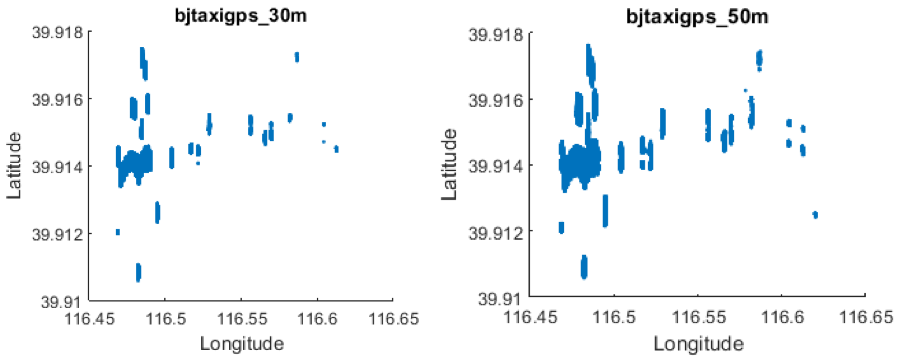
\includegraphics{30m_50m}
\centering
\caption{Plot of data points after outlier removal}\label{Fig:after_removal}
\end{figure}

After the outliers were removed, two data sets remained. They are hereinafter referred to as \emph{bjtaxigps\_30m}, where outliers were filtered by a threshold of 30 metres and \emph{bjtaxigps\_50m}, where outliers were filtered by a threshold of 50 metres, respectively. bjtaxigps\_30m contains approximately 51 million records while bjtaxigps\_50m has 59 million. All algorithms described hereinafter are applicable to both data sets. Figure~\ref{Fig:after_removal} gives a plot of the data points from both data sets. Clearly, the data points are now contained in a much smaller area and roughly form a shape similar to that of the street they are mapped to. 